% -*- TeX-master: "sicp.tex" -*-
\section{The Elements of Programming}
\label{sec:1.1}

A powerful programming language is more than just a means for
instructing a computer to perform tasks.  The language also serves as
a framework within which we organize our ideas about processes.  Thus,
when we describe a language, we should pay particular attention to the
means that the language provides for combining simple ideas to form
more complex ideas.  Every powerful language has three mechanisms for
accomplishing this:

\begin{description}
\item[primitive expressions], which represent the simplest entities
  the language is concerned with,
\item[means of combination], by which compound elements are built from
  simpler ones, and
\item[means of abstraction], by which compound elements can be named
  and manipulated as units.
\end{description}


In programming, we deal with two kinds of elements: \idef{procedures}
and \idef{data}. (Later we will discover that they are really not so
distinct.)  Informally, data is ``stuff'' that we want to manipulate,
and procedures are descriptions of the rules for manipulating the
data.  Thus, any powerful programming language should be able to
describe primitive data and primitive procedures and should have
methods for combining and abstracting procedures and data.

In this chapter we will deal only with simple numerical data so that
we can focus on the rules for building procedures.\footnote{The
  characterization of numbers as ``simple data'' is a barefaced bluff.
  In fact, the treatment of numbers is one of the trickiest and most
  confusing aspects of any programming language.  Some typical issues
  involved are these: Some computer systems distinguish
  \textit{integers}, such as 2, from \textit{real numbers}, such as
  2.71.  Is the real number 2.00 different from the integer 2?  Are
  the arithmetic operations used for integers the same as the
  operations used for real numbers?  Does 6 divided by 2 produce 3, or
  3.0?  How large a number can we represent?  How many decimal places
  of accuracy can we represent?  Is the range of integers the same as
  the range of real numbers?  Above and beyond these questions, of
  course, lies a collection of issues concerning roundoff and
  truncation errors -- the entire science of numerical analysis.
  Since our focus in this book is on large-scale program design rather
  than on numerical techniques, we are going to ignore these problems.
  The numerical examples in this chapter will exhibit the usual
  roundoff behavior that one observes when using arithmetic operations
  that preserve a limited number of decimal places of accuracy in
  noninteger operations.} In later chapters we will see that these
same rules allow us to build procedures to manipulate compound data as
well.

\subsection{Expressions}
\label{sec:1.1.1}

One easy way to get started at programming is to examine some typical
interactions with an interpreter for the Scheme dialect of Lisp.
Imagine that you are sitting at a computer terminal.  You type an
\idef{expression}, and the interpreter responds by displaying the result of
its \idef{evaluating} that expression.

One kind of primitive expression you might type is a number.  (More
precisely, the expression that you type consists of the numerals that
represent the number in base 10.)  If you present Lisp with
a number

\texttt{486}

\noindent
the interpreter will respond by printing\footnote{Throughout this
  book, when we wish to emphasize the distinction between the input
  typed by the user and the response printed by the interpreter, we
  will show the latter in slanted characterization}\relax

\texttt{\textit{486}}

\noindent Expressions representing numbers may be combined with an
expression representing a primitive procedure (such as \texttt{+} or
\texttt{*}) to form a compound expression that represents the
application of the procedure to those numbers.  For example:

\begin{verbatim}
% TODO: Convert to a typescript environment
> (+ 137 349)
486
> (- 1000 334)
666
> (* 5 99)
495
> (/ 10 5)
2
> (+ 2.7 10)
12.7
\end{verbatim}

Expressions such as these, formed by delimiting a list of expressions
within parentheses in order to denote procedure application, are
called combinations.  The leftmost element in the list is called the
\idef{operator}, and the other elements are called \idef{operands}.
The value of a combination is obtained by applying the procedure
specified by the operator to the \idef{arguments} that are the values of the
operands.

The convention of placing the operator to the left of the operands is
known as \idef{prefix notation}, and it may be somewhat confusing at
first because it departs significantly from the customary mathematical
convention.  Prefix notation has several advantages, however.  One of
them is that it can accommodate procedures that may take an arbitrary
number of arguments, as in the following examples:

\begin{verbatim}
% TODO: Convert to a typescript environment
> (+ 21 35 12 7)
75
> (* 25 4 12)
1200
\end{verbatim}

No ambiguity can arise, because the operator is always the leftmost
element and the entire combination is delimited by the parentheses.

A second advantage of prefix notation is that it extends in a
straightforward way to allow combinations to be \textbf{nested}, that
is, to have combinations whose elements are themselves
combinations:

\begin{verbatim}
% TODO: Convert to a typescript environment
> (+ (* 3 5) (- 10 6))
19
\end{verbatim}

There is no limit (in principle) to the depth of such nesting and to
the overall complexity of the expressions that the Lisp interpreter
can evaluate.  It is we humans who get confused by still relatively
simple expressions such as

\begin{verbatim}
> (+ (* 3 (+ (* 2 4) (+ 3 5))) (+ (- 10 7) 6))
\end{verbatim}

\noindent which the interpreter would readily evaluate to be 57.  We can help
ourselves by writing such an expression in the form

\begin{schemedisplay}
(+ (* 3
      (+ (* 2 4)
         (+ 3 5)))
   (+ (- 10 7)
      6))
\end{schemedisplay}

\noindent following a formatting convention known as
\idef{pretty-printing}, in which each long combination is written so
that the operands are aligned vertically.  The resulting indentations
display clearly the structure of the expression. \footnote{Lisp
  systems typically provide features to aid the user in formatting
  expressions.  Two especially useful features are one that
  automatically indents to the proper pretty-print position whenever a
  new line is started and one that highlights the matching left
  parenthesis whenever a right parenthesis is typed.}

Even with complex expressions, the interpreter always operates in the
same basic cycle: It reads an expression from the terminal, evaluates
the expression, and prints the result.  This mode of operation is
often expressed by saying that the interpreter runs in a
\idef{read-eval-print loop}.  Observe in particular that it is not
necessary to explicitly instruct the interpreter to print the value of
the expression.\footnote{Lisp obeys the convention that every
  expression has a value. This convention, together with the old
  reputation of Lisp as an inefficient language, is the source of the
  quip by Alan Perlis (paraphrasing Oscar Wilde) that ``Lisp
  programmers know the value of everything but the cost of nothing.''}

\subsection{Naming and the Environment}
\label{sec:1.1.2}

A critical aspect of a programming language is the means it provides
for using names to refer to computational objects.  We say that the
name identifies a \idef{variable} whose \idef{value} is the object.

In the Scheme dialect of Lisp, we name things with \idef{define}.
Typing

\begin{verbatim}
> (define size 2)
\end{verbatim}

\noindent causes the interpreter to associate the value 2 with the
name \texttt{size}.\footnote{In this book, we do not show the
  interpreter's response to evaluating definitions, since this is
  highly implementation-dependent.}  Once the name \texttt{size} has
been associated with the number 2, we can refer to the value 2 by
name:

\begin{verbatim}
> size
2
> (* 5 size)
10
\end{verbatim}

Here are further examples of the use of \texttt{define}:

\begin{verbatim}
> (define pi 3.14159)
> (define radius 10)
> (* pi (* radius radius))
314.159
> (define circumference (* 2 pi radius))
> circumference
62.8318
\end{verbatim}

\texttt{Define} is our language's simplest means of abstraction, for
it allows us to use simple names to refer to the results of compound
operations, such as the \texttt{circumference} computed above.  In
general, computational objects may have very complex structures, and
it would be extremely inconvenient to have to remember and repeat
their details each time we want to use them.  Indeed, complex programs
are constructed by building, step by step, computational objects of
increasing complexity. The interpreter makes this step-by-step program
construction particularly convenient because name-object associations
can be created incrementally in successive interactions.  This feature
encourages the incremental development and testing of programs and is
largely responsible for the fact that a Lisp program usually consists
of a large number of relatively simple procedures.

It should be clear that the possibility of associating values with
symbols and later retrieving them means that the interpreter must
maintain some sort of memory that keeps track of the name-object
pairs.  This memory is called the \idef{environment} (more precisely
the \idef{global environment}, since we will see later that a
computation may involve a number of different environments).\footnote{
  \ref{chap:3} will show that this notion of environment is crucial,
  both for understanding how the interpreter works and for
  implementing interpreters.}

\subsection{Evaluating Combinations}
\label{sec:1.1.3}

One of our goals in this chapter is to isolate issues about thinking
procedurally.  As a case in point, let us consider that, in evaluating
combinations, the interpreter is itself following a procedure.

% TODO: Improve this formatting.
To evaluate a combination, do the following:

\begin{enumerate}
\item Evaluate the subexpressions of the combination.<p>

\item Apply the procedure that is the value of the leftmost 
subexpression (the operator) to the arguments that are the values of
the other subexpressions (the operands).
\end{enumerate}

Even this simple rule illustrates some important points about
processes in general.  First, observe that the first step dictates
that in order to accomplish the evaluation process for a combination
we must first perform the evaluation process on each element of the
combination.  Thus, the evaluation rule is \idef{recursive} in nature;
that is, it includes, as one of its steps, the need to invoke the rule
itself.\footnote{ It may seem strange that the evaluation rule says,
  as part of the first step, that we should evaluate the leftmost
  element of a combination, since at this point that can only be an
  operator such as \texttt{+} or \texttt{*} representing a built-in
  primitive procedure such as addition or multiplication.  We will see
  later that it is useful to be able to work with combinations whose
  operators are themselves compound expressions.}

Notice how succinctly the idea of recursion can be used to express
what, in the case of a deeply nested combination, would otherwise be
viewed as a rather complicated process.  For example, evaluating

\begin{schemedisplay}
(* (+ 2 (* 4 6))
   (+ 3 5 7))
\end{schemedisplay}

\noindent requires that the evaluation rule be applied to four
different combinations.  We can obtain a picture of this process by
representing the combination in the form of a tree, as shown in figure
% TODO: debug why this shows up as 1.3
\ref{fig:1.1}.  Each combination is represented by a node with
branches corresponding to the operator and the operands of the
combination stemming from it.  The terminal nodes (that is, nodes with
no branches stemming from them) represent either operators or numbers.
Viewing evaluation in terms of the tree, we can imagine that the
values of the operands percolate upward, starting from the terminal
nodes and then combining at higher and higher levels.  In general, we
shall see that recursion is a very powerful technique for dealing with
hierarchical, treelike objects.  In fact, the ``percolate values
upward'' form of the evaluation rule is an example of a general kind
of process known as \idef{tree accumulation}.

\begin{figure}
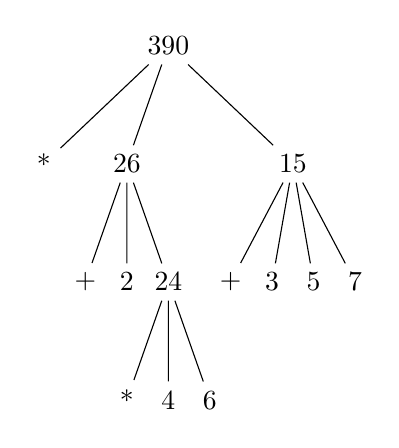
\begin{tikzpicture}
  % TODO: Improve this diagram
  [level 1/.style={sibling distance=3em},
   level 2/.style={sibling distance=1.5em}]
  \node {390}
    child { node {*} }
    child { node {26}
      child { node {+} }
      child { node {2} }
      child { node {24}
        child { node {*} }
        child { node {4} }
        child { node {6} } } }
    child[missing] {}
    child { node {15}
      child { node {+} }
      child { node {3} }
      child { node {5} }
      child { node {7} } } ;
\end{tikzpicture}
\caption{Tree representation, showing the value of each subcombination.}
\label{fig:1.1} % TODO: This should label the figure rather than the section.
\end{figure}

Next, observe that the repeated application of the first step brings
us to the point where we need to evaluate, not combinations, but
primitive expressions such as numerals, built-in operators, or other
names.  We take care of the primitive cases by stipulating that

\begin{itemize}
\item the values of numerals are the numbers that they name,
\item the values of built-in operators are the machine instruction
  sequences that carry out the corresponding operations, and
\item the values of other names are the objects associated with those
  names in the environment.
\end{itemize}

We may regard the second rule as a special case of the third one by
stipulating that symbols such as \texttt{+} and \texttt{*} are also
included in the global environment, and are associated with the
sequences of machine instructions that are their ``values.''  The key
point to notice is the role of the environment in determining the
meaning of the symbols in expressions.  In an interactive language
such as Lisp, it is meaningless to speak of the value of an expression
such as \texttt{(+ x 1)} without specifying any information about the
environment that would provide a meaning for the symbol \texttt{x} (or
even for the symbol \texttt{+}).  As we shall see in \ref{chap:3}, the
general notion of the environment as providing a context in which
evaluation takes place will play an important role in our
understanding of program execution.

Notice that the evaluation rule given above does not handle
definitions.  For instance, evaluating \texttt{(define x 3)} does not
apply \texttt{define} to two arguments, one of which is the value of
the symbol \texttt{x} and the other of which is 3, since the purpose
of the \texttt{define} is precisely to associate \texttt{x} with a
value.  (That is, \texttt{(define x 3)} is not a combination.)

Such exceptions to the general evaluation rule are called
special forms.  \texttt{Define} is the only example of a
special form that we have seen so far, but we will meet others
shortly.  Each special form has its own evaluation rule. The various
kinds of expressions (each with its associated evaluation rule)
constitute the \idef{syntax} of the programming language.  In
comparison with most other programming languages, Lisp has a very
simple syntax; that is, the evaluation rule for expressions can be
described by a simple general rule together with specialized rules for
a small number of special forms.\footnote{Special syntactic forms that
  are simply convenient alternative surface structures for things that
  can be written in more uniform ways are sometimes called
  \idef{syntactic sugar}, to use a phrase coined by Peter Landin.  In
  comparison with users of other languages, Lisp programmers, as a
  rule, are less concerned with matters of syntax.  (By contrast,
  examine any Pascal manual and notice how much of it is devoted to
  descriptions of syntax.)  This disdain for syntax is due partly to
  the flexibility of Lisp, which makes it easy to change surface
  syntax, and partly to the observation that many ``convenient''
  syntactic constructs, which make the language less uniform, end up
  causing more trouble than they are worth when programs become large
  and complex.  In the words of Alan Perlis, ``Syntactic sugar causes
  cancer of the semicolon.''}

\subsection{Compound Procedures}
\label{sec:1.1.4}

We have identified in Lisp some of the elements that must appear in
any powerful programming language:

\begin{itemize}
\item Numbers and arithmetic operations are 
primitive data and procedures.
\item Nesting of combinations provides a means of 
combining operations.
\item Definitions that associate names with values provide a
limited means of abstraction.
\end{itemize}

Now we will learn about
\idef{procedure definitions}, a much more powerful abstraction
technique by which a compound operation can be given a name and then
referred to as a unit.

We begin by examining how to express the idea of ``squaring.''  We
might say, ``To square something, multiply it by itself.''  This is
expressed in our language as 

\begin{schemedisplay}
> (define (square x) (* x x))
\end{schemedisplay}

We can understand this in the following way:

% TODO: Fill in this diagram
\begin{tabular}{cccccc}
  $\texttt{(define}$ & $\texttt{(square}$ & $\texttt{x)}$ & $\texttt{(*}$ & $\texttt{x}$ & $\texttt{x))}$ \\
  $\uparrow{}$ & $\uparrow{}$ & $\uparrow{}$ & $\uparrow{}$ & $\uparrow{}$ & $\uparrow{}$ \\
  To & square & something, & multiply & it & by itself.
\end{tabular}

We have here a \idef{compound procedure}, which has been given the
name \texttt{square}.  The procedure represents the operation of
multiplying something by itself.  The thing to be multiplied is given
a local name, \texttt{x}, which plays the same role that a pronoun
plays in natural language.  Evaluating the definition creates this
compound procedure and associates it with the name \texttt{square}.
\footnote{Observe that there are two different operations being
  combined here: we are creating the procedure, and we are giving it
  the name \texttt{square}.  It is possible, indeed important, to be
  able to separate these two notions -- to create procedures without
  naming them, and to give names to procedures that have already been
  created.  We will see how to do this in section \ref{sec:1.3.2}.}


The general form of a procedure definition is

\begin{schemedisplay}
(define (<name> <formal parameters>) <body>)
\end{schemedisplay}

The \slot{name}; is a symbol to be associated with the procedure
definition in the environment.\footnote{Throughout this book, we will
  describe the general syntax of expressions by using italic symbols
  delimited by angle brackets -- e.g. \slot{name} -- to denote the
  ``slots'' in the expression to be filled in when such an expression
  is actually used.} The \slot{formal parameters} are the names used
within the body of the procedure to refer to the corresponding
arguments of the procedure.  The \slot{body} is an expression that
will yield the value of the procedure application when the formal
parameters are replaced by the actual arguments to which the procedure
is applied.\footnote{More generally, the body of the procedure can be
  a sequence of expressions.  In this case, the interpreter evaluates
  each expression in the sequence in turn and returns the value of the
  final expression as the value of the procedure application.}  The
\slot{name} and the \slot{formal parameters} are grouped within
parentheses, just as they would be in an actual call to the procedure
being defined.

Having defined \texttt{square}, we can now use it:

\begin{verbatim}
> (square 21)
441
> (square (+ 2 5))
49
> (square (square 3))
81
\end{verbatim}

We can also use \texttt{square} as a building block in defining other
procedures.  For example, $x^2 + y^2$

\begin{verbatim}
> (+ (square x) (square y))
\end{verbatim}

We can easily define a procedure \texttt{sum-of-squares} that, given
any two numbers as arguments, produces the sum of their squares:

\begin{verbatim}
>(define (sum-of-squares x y)
>  (+ (square x) (square y)))

> (sum-of-squares 3 4)
25
\end{verbatim}

Now we can use \texttt{sum-of-squares} as a building block in constructing
further procedures:

\begin{verbatim}
> (define (f a)
>  (sum-of-squares (+ a 1) (* a 2)))

> (f 5)
136
\end{verbatim}

Compound procedures are used in exactly the same way as primitive
procedures.  Indeed, one could not tell by looking at the definition
of \texttt{sum-of-squares} given above whether \texttt{square} was
built into the interpreter, like \texttt{+} and \texttt{*}, or defined
as a compound procedure.

\subsection{The Substitution Model for Procedure Application}
\label{sec:1.1.5}

To evaluate a combination whose operator names a compound procedure, the
interpreter follows much the same process as for combinations whose
operators name primitive procedures, which we described in
section \ref{sec:1.1.3}.  That is, the interpreter
evaluates the elements of the combination and applies the procedure
(which is the value of the operator of the combination) to the
arguments (which are the values of the operands of the combination).

We can assume that the mechanism for applying primitive procedures to
arguments is built into the interpreter.  For compound procedures, the
application process is as follows:

% TODO: Format this as pseudocode
\begin{verbatim}
To apply a compound procedure to arguments, evaluate the body of
the procedure with each formal parameter replaced by the
corresponding argument.
\end{verbatim}

To illustrate this process, let's evaluate the combination

\begin{schemedisplay}
(f 5)
\end{verbatim}

where \texttt{f} is the procedure defined in
section \ref{sec:1.1.4}.  We begin by retrieving the
body of \texttt{f}

\begin{schemedisplay}
(sum-of-squares (+ a 1) (* a 2))
\end{schemedisplay}

Then we replace the formal parameter \texttt{a} by the argument 5:

\begin{schemedisplay}
(sum-of-squares (+ 5 1) (* 5 2))
\end{schemedisplay}

Thus the problem reduces to the evaluation of a combination with two
operands and an operator \texttt{sum-of-squares}.  Evaluating this
combination involves three subproblems.  We must evaluate the operator
to get the procedure to be applied, and we must evaluate the operands
to get the arguments.  Now \texttt{(+ 5 1)} produces 6 and \texttt{(*
  5 2)} produces 10, so we must apply the \texttt{sum-of-squares}
procedure to 6 and 10.  These values are substituted for the formal
parameters \texttt{x} and \texttt{y} in the body of
\texttt{sum-of-squares}, reducing the expression to

\begin{schemedisplay}
(+ (square 6) (square 10))
\end{schemedisplay}

If we use the definition of \texttt{square}, this reduces to

\begin{schemedisplay}
(+ (* 6 6) (* 10 10))
\end{schemedisplay}

which reduces by multiplication to


\begin{schemedisplay}
(+ 36 100)
\end{schemedisplay}

and finally to

\begin{schemedisplay}
136
\end{schemedisplay}

The process we have just described is called the \textit{substitution
model} for procedure application.  It can be taken as a model that
determines the ``meaning'' of procedure application, insofar as the
procedures in this chapter are concerned.  However, there are two
points that should be stressed:

\begin{itemize}
\item The purpose of the substitution is to help us think about procedure
application, not to provide a description of how the interpreter
really works.  Typical interpreters do not evaluate procedure
applications by manipulating the text of a procedure to substitute
values for the formal parameters.  In practice, the ``substitution''
is accomplished by using a local environment for the formal
parameters.  We will discuss this more fully in chapters 3 and 4 when
we examine the implementation of an interpreter in detail.

\item Over the course of this book, we will present a sequence of
  increasingly elaborate models of how interpreters work, culminating
  with a complete implementation of an interpreter and compiler in
  chapter 5.  The substitution model is only the first of these models
  -- a way to get started thinking formally about the evaluation
  process.  In general, when modeling phenomena in science and
  engineering, we begin with simplified, incomplete models.  As we
  examine things in greater detail, these simple models become
  inadequate and must be replaced by more refined models.  The
  substitution model is no exception.  In particular, when we address
  in chapter 3 the use of procedures with ``mutable data,'' we will
  see that the substitution model breaks down and must be replaced by
  a more complicated model of procedure application.\footnote{Despite
    the simplicity of the substitution idea, it turns out to be
    surprisingly complicated to give a rigorous mathematical
    definition of the substitution process.  The problem arises from
    the possibility of confusion between the names used for the formal
    parameters of a procedure and the (possibly identical) names used
    in the expressions to which the procedure may be applied.  Indeed,
    there is a long history of erroneous definitions of
    \textit{substitution} in the literature of logic and programming
    semantics.  See Stoy 1977 for a careful discussion of
    substitution.}
\end{itemize}

\subsection*{Applicative order versus normal order}

According to the description of evaluation given in section
\ref{sec:1.1.3}, the interpreter first evaluates the operator and operands
and then applies the resulting procedure to the resulting arguments.
This is not the only way to perform evaluation.  An alternative
evaluation model would not evaluate the operands until their values
were needed.  Instead it would first substitute operand expressions
for parameters until it obtained an expression involving only
primitive operators, and would then perform the evaluation.  If we
used this method, the evaluation of

\begin{schemedisplay}
(f 5)
\end{schemedisplay}

\noindent would proceed according to the sequence of expansions

\begin{schemedisplay}
(sum-of-squares (+ 5 1) (* 5 2))

(+    (square (+ 5 1))      (square (* 5 2))  )

(+    (* (+ 5 1) (+ 5 1))   (* (* 5 2) (* 5 2)))
\end{schemedisplay}

\noindent followed by the reductions

\begin{schemedisplay}
(+         (* 6 6)             (* 10 10))

(+           36                   100)

                    136
\end{schemedisplay}

This gives the same answer as our previous evaluation model, but the
process is different.  In particular, the evaluations
of \texttt{(+ 5 1)} and \texttt{(* 5 2)} are each performed twice here,
corresponding to the reduction of the expression

\begin{schemedisplay}
(* x x)
\end{schemedisplay}

\noindent with \texttt{x} replaced respectively by \texttt{(+ 5 1)} and \texttt{(* 5 2)}.

This alternative ``fully expand and then reduce'' evaluation method is
known as \idef{normal-order evaluation}, in contrast to the ``evaluate
the arguments and then apply'' method that the interpreter actually
uses, which is called \idef{applicative-order evaluation}.  It can be
shown that, for procedure applications that can be modeled using
substitution (including all the procedures in the first two chapters
of this book) and that yield legitimate values, normal-order and
applicative-order evaluation produce the same value.  (See exercise
\ref{exc:1.5} for an instance of an ``illegitimate'' value where
normal-order and applicative-order evaluation do not give the same
result.)

Lisp uses applicative-order evaluation, partly because of the
additional efficiency obtained from avoiding multiple evaluations of
expressions such as those illustrated with \texttt{(+ 5 1)} and
\texttt{(* 5 2)} above and, more significantly, because normal-order
evaluation becomes much more complicated to deal with when we leave
the realm of procedures that can be modeled by substitution.  On the
other hand, normal-order evaluation can be an extremely valuable tool,
and we will investigate some of its implications in chapters 3 and
4.\footnote{In chapter 3, we will introduce \textit{stream
    processing}, which is a way of handling apparently ``infinite''
  data structures by incorporating a limited form of normal-order
  evaluation.  In section \ref{sec:4.2} we will modify the scheme
  interpreter to produce a normal-order variant of Scheme.}

\subsection{Conditional Expressions and Predicates}
\label{sec:1.1.6}

The expressive power of the class of procedures that we can define at
this point is very limited, because we have no way to make tests and
to perform different operations depending on the result of a test.
For instance, we cannot define a procedure that computes the absolute
value of a number by testing whether the number is positive, negative,
or zero and taking different actions in the different cases according
to the rule

\begin{equation*}
  % TODO: Format this equation nicely
  |x| = 
    \begin{cases}
       \quad x & \text{if } x > 0 \\
       \quad 0 & \text{if } x = 0 \\
       -x & \text{if } x < 0
    \end{cases}
\end{equation*}

This construct is called a \idef{case analysis}, and
there is a special form in Lisp for notating such a case
analysis.  It is called \texttt{cond} (which stands for
``conditional''), and it is used as follows:

\begin{schemedisplay}
(define (abs x)
  (cond ((> x 0) x)
        ((= x 0) 0)
        ((< x 0) (- x))))
\end{schemedisplay}

The general form of a conditional expression is

\begin{schemedisplay}
% TODO: Format this properly
(cond (<<em>p_1</em>> <<em>e_1</em>>)
      (<<em>p_2</em>> <<em>e_2</em>>)
      <img src="book-Z-G-D-18.gif" border="0">
      (<<em>p_{<em>n</em>}</em>> <<em>e_{<em>n</em>}</em>>))
\end{schemedisplay}

consisting of the symbol \texttt{cond} followed by parenthesized pairs
of expressions \texttt{(\slot{p} \slot{e})} called \idef{clauses}. The
first expression in each pair is a \idef{predicate} -- that is, an
expression whose value is interpreted as either true or
false.\footnote{``Interpreted as either true or false'' means this: In
  Scheme, there are two distinguished values that are denoted by the
  constants \texttt{\#t} and \texttt{\#f}.  When the interpreter checks
  a predicate's value, it interprets \texttt{\#f} as false.  Any other
  value is treated as true.  (Thus, providing \texttt{\#t} is logically
  unnecessary, but it is convenient.)  In this book we will use names
  \texttt{true} and \texttt{false}, which are associated with the
  values \texttt{\#t} and \texttt{\#f} respectively.}


\idef{Conditional expressions} are evaluated as follows.  The predicate
\slot{p_1} is evaluated first.  If its value is false, then
\slot{p_2} is evaluated.  If \slot{p_2}'s value is also false, then
\slot{p_3} is evaluated.  This process continues until a predicate is
found whose value is true, in which case the interpreter returns the
value of the corresponding \idef{consequent expression} \slot{e} of the
clause as the value of the conditional expression.  If none of the
\slot{p}'s is found to be true, the value of the \texttt{cond} is
undefined.

The word \idef{predicate} is used for procedures that return true or
false, as well as for expressions that evaluate to true or false.  The
absolute-value procedure \texttt{abs} makes use of the
\index{primitive}primitive predicates \texttt{$>$}, \texttt{$<$}, and
\texttt{=}.\footnote{\texttt{abs} also uses the ``minus'' operator
  \texttt{-}, which, when used with a single operand, as in \texttt{(-
    x)}, indicates negation.}  These take two numbers as arguments and
test whether the first number is, respectively, greater than, less
than, or equal to the second number, returning true or false
accordingly.

Another way to write the absolute-value procedure is

\begin{schemedisplay}
(define (abs x)
  (cond ((< x 0) (- x))
        (else x)))
\end{schemedisplay}

\noindent which could be expressed in English as ``If $x$ is less than
zero return $-x$; otherwise return $x$.''  \texttt{Else} is a special
symbol that can be used in place of the \slot{p} in the final clause
of a \texttt{cond}.  This causes the \texttt{cond} to return as its
value the value of the corresponding \slot{e} whenever all previous
clauses have been bypassed.  In fact, any expression that always
evaluates to a true value could be used as the \slot{p} here.

Here is yet another way to write the absolute-value procedure:

\begin{schemedisplay}
(define (abs x)
  (if (< x 0)
      (- x)
      x))
\end{schemedisplay}

This uses the special form \texttt{if}, a restricted type of conditional
that can be used when there are precisely two cases in the case
analysis.  The general form of an \texttt{if} expression is

\begin{schemedisplay}
(if \slot{predicate} \slot{consequent} \slot{alternative})
\end{schemedisplay}

To evaluate an \texttt{if} expression, the interpreter starts by
evaluating the \slot{predicate} part of the expression.  If the
\slot{predicate} evaluates to a true value, the interpreter then
evaluates the \slot{consequent} and returns its value.  Otherwise it
evaluates the \slot{alternative} and returns its value.\footnote{A
  minor difference between \texttt{if} and \texttt{cond} is that the
  \slot{e} part of each \texttt{cond} clause may be a sequence of
  expressions. If the corresponding \slot{p} is found to be true, the
  expressions \slot{e} are evaluates in sequence and the value of the
  final expression in the sequence is returned as the value of the
  \texttt{cond}. In an \texttt{if} expression, however, the
  \slot{consequent} and \slot{alternative} must be single
  expressions.}

In addition to primitive predicates such as \texttt{<}, \texttt{=},
and \texttt{>}, there are logical composition operations, which enable
us to construct compound predicates.  The three most frequently used
are these:

\begin{itemize}
\item \texttt{(and \slot{e_1} \ldots{} \slot{e_n})}

The interpreter evaluates the expressions \slot{e} one at a time, in
left-to-right order.  If any \slot{e} evaluates to false, the value of
the \texttt{and} expression is false, and the rest of the \slot{e}'s
are not evaluated.  If all \slot{e}'s evaluate to true values, the
value of the \texttt{and} expression is the value of the last one.

\item \texttt{(or \slot{e_1} \ldots{} \slot{e_n})}

The interpreter evaluates the expressions \slot{e} one at a time, in
left-to-right order.  If any \slot{e} evaluates to a true value, that
value is returned as the value of the \texttt{or} expression, and the
rest of the \slot{e}'s are not evaluated.  If all \slot{e}'s evaluate
to false, the value of the \texttt{or} expression is false.

\item \texttt{(not \slot{e})}

The value of a \texttt{not} expression is true
when the expression \slot{e} evaluates to false, and false otherwise.
\end{itemize}

Notice that \texttt{and} and \texttt{or} are special forms, not
procedures, because the subexpressions are not necessarily all
evaluated.  \texttt{Not} is an ordinary procedure.

As an example of how these are used, the condition that a number
$x$ be in the range $5 < x < 10$ may be expressed as

\begin{schemedisplay}
(and (> x 5) (< x 10))
\end{schemedisplay}

As another example, we can define a predicate to test whether one
number is greater than or equal to another as

\begin{schemedisplay}
(define (>= x y)
  (or (> x y) (= x y)))
\end{schemedisplay}

\noindent or alternatively as

\begin{schemedisplay}
(define (>= x y)
  (not (< x y)))
\end{schemedisplay}

\begin{Exercise}
  \label{exc:1.1}
Below is a sequence of expressions.  What is the result printed by the
interpreter in response to each expression?  Assume that the sequence
is to be evaluated in the order in which it is presented.

\begin{schemedisplay}
10
(+ 5 3 4)
(- 9 1)
(/ 6 2)
(+ (* 2 4) (- 4 6))
(define a 3)
(define b (+ a 1))
(+ a b (* a b))
(= a b)
(if (and (> b a) (< b (* a b)))
    b
    a)
(cond ((= a 4) 6)
      ((= b 4) (+ 6 7 a))
      (else 25))
(+ 2 (if (> b a) b a))
(* (cond ((> a b) a)
         ((< a b) b)
         (else -1))
   (+ a 1))
\end{schemedisplay}
\end{Exercise}

\begin{Exercise}
\label{exc:1.2}
Translate the following expression into prefix form
\begin{equation*}
  \frac{5 + 4 + 3 + (2 - (3 - (6 + \frac{4}{5})))}
  {3 (6-2) (2-7)}
\end{equation*}
\end{Exercise}

\begin{Exercise}
\label{exc:1.3}
Define a procedure that takes three numbers as arguments and returns
the sum of the squares of the two larger numbers.
\end{Exercise}

\begin{Exercise}
\label{exc:1.4}
Observe that our model of evaluation allows for combinations whose
operators are compound expressions.  Use this observation to
describe the behavior of the following procedure:
\begin{schemedisplay}
(define (a-plus-abs-b a b)
  ((if (> b 0) + -) a b))
\end{schemedisplay}
\end{Exercise}

\begin{Exercise}
\label{exc:1.5}
Ben Bitdiddle has invented a test to determine whether the interpreter
he is faced with is using applicative-order evaluation or normal-order
evaluation.  He defines the following two procedures:

\begin{schemedisplay}
(define (p) (p))

(define (test x y)
  (if (= x 0)
      0
      y))
\end{schemedisplay}

Then he evaluates the expression

\begin{schemedisplay}
(test 0 (p))
\end{schemedisplay}

What behavior will Ben observe with an interpreter that uses
applicative-order evaluation?  What behavior will he observe with an
interpreter that uses normal-order evaluation?  Explain your answer.
(Assume that the evaluation rule for the special form \texttt{if} is
the same whether the interpreter is using normal or applicative order:
The predicate expression is evaluated first, and the result determines
whether to evaluate the consequent or the alternative expression.)
\end{Exercise}

\subsection{Example: Square Roots by Newton's Method}
\label{sec:1.1.7}

Procedures, as introduced above, are much like ordinary mathematical
functions.  They specify a value that is determined by one or more
parameters.  But there is an important difference between
mathematical functions and computer procedures.  Procedures must be
effective.

As a case in point, consider the problem of computing square
roots.  We can define the square-root function as

\begin{displaymath}
  \sqrt{x} = \mathrm{the}~ y ~\mathrm{such~that}~ y \ge 0 ~\mathrm{and}~ {y^2} = x
\end{displaymath}

This describes a perfectly legitimate mathematical function.  We could
use it to recognize whether one number is the square root of another, or
to derive facts about square roots in general.  On the other hand, the
definition does not describe a procedure.  Indeed, it tells us almost
nothing about how to actually find the square root of a given number.  It
will not help matters to rephrase this definition in pseudo-Lisp:

\begin{schemedisplay}
(define (sqrt x)
  (the y (and (>= y 0)
              (= (square y) x))))
\end{schemedisplay}

This only begs the question.

The contrast between function and procedure is a reflection of the
general distinction between describing properties of things and
describing how to do things, or, as it is sometimes referred to, the
distinction between declarative knowledge and imperative knowledge.
In mathematics we are usually concerned with declarative (what is)
descriptions, whereas in computer science we are usually concerned
with imperative (how to) descriptions.\footnote{ Declarative and
  imperative descriptions are intimately related, as indeed are
  mathematics and computer science.  For instance, to say that the
  answer produced by a program is ``correct'' is to make a declarative
  statement about the program.  There is a large amount of research
  aimed at establishing techniques for proving that programs are
  correct, and much of the technical difficulty of this subject has to
  do with negotiating the transition between imperative statements
  (from which programs are constructed) and declarative statements
  (which can be used to deduce things).  In a related vein, an
  important current area in programming-language design is the
  exploration of so-called very high-level languages, in which one
  actually programs in terms of declarative statements.  The idea is
  to make interpreters sophisticated enough so that, given ``what is''
  knowledge specified by the programmer, they can generate ``how to''
  knowledge automatically.  This cannot be done in general, but there
  are important areas where progress has been made.  We shall revisit
  this idea in chapter \ref{chap:4}.}


How does one compute square roots?  The most common way is to use
Newton's method of successive approximations, which says that whenever
we have a guess $y$ for the value of the square root of a number $x$,
we can perform a simple manipulation to get a better guess (one closer
to the actual square root) by averaging $y$ with
$\frac{x}{y}$.\footnote{This square-root algorithm is actually a
  special case of Newton's method, which is a general technique for
  finding roots of equations.  The square-root algorithm itself was
  developed by Heron of Alexandria in the first century \textsc{a.d}.
  We will see how to express the general Newton's method as a Lisp
  procedure in section \ref{sec:1.3.4}.}  For example, we can compute
the square root of 2 as follows.  Suppose our initial guess is 1:

\begin{tabular}{|c|c|c|}
  \hline{}
  Guess & Quotient & Average \\
  \hline{}
  1 & $2/1 = 2$ & $\frac{2+1}{2} = 1.5$ \\
  1.5 & $\frac{2}{1.5} = 1.3333$ & $\frac{1.3333 + 1.5}{2} = 1.4167$ \\
  1.4167 & $\frac{2}{1.4167} = 1.4118$ & $\frac{1.4167 + 1.4118}{2} = 1.4142$ \\
  1.4142 & \ldots & \ldots \\
  \hline{}
  % TODO: Fix the lines coming out of the bottom of this table.
\end{tabular}

Continuing this process, we obtain better and better
approximations to the square root.

Now let's formalize the process in terms of procedures.  We start with
a value for the radicand (the number whose square root we are trying
to compute) and a value for the guess.  If the guess is good enough
for our purposes, we are done; if not, we must repeat the process with an
improved guess.  We write this basic strategy as a procedure:

\begin{schemedisplay}
(define (sqrt-iter guess x)
  (if (good-enough? guess x)
      guess
      (sqrt-iter (improve guess x)
                 x)))
\end{schemedisplay}

A guess is improved by averaging
it with the quotient of the radicand and the old guess:

\begin{schemedisplay}
(define (improve guess x)
  (average guess (/ x guess)))
\end{schemedisplay}

\noindent where

\begin{schemedisplay}
(define (average x y)
  (/ (+ x y) 2))
\end{schemedisplay}

We also have to say what we mean by ``good enough.''  The following
will do for illustration, but it is not really a very good test.  (See
exercise \ref{exc:1.7}.)  The idea is to improve the answer until it
is close enough so that its square differs from the radicand by less
than a predetermined tolerance (here 0.001):\footnote{We will usually
  give predicates names ending with question marks, to help us
  remember that they are predicates.  This is just a stylistic
  convention.  As far as the interpreter is concerned, the question
  mark is just an ordinary character.}

\begin{schemedisplay}
(define (good-enough? guess x)
  (< (abs (- (square guess) x)) 0.001))
\end{schemedisplay}

Finally, we need a way to get started.  For instance, we can always
guess that the square root of any number is 1:\footnote{Observe that
  we express our initial guess as 1.0 rather than 1.  This would not
  make any difference in many Lisp implementations. MIT Scheme,
  however, distinguishes between exact integers and decimal values,
  and dividing two integers produces a rational number rather than a
  decimal.  For example, dividing 10 by 6 yields 5/3, while dividing
  10.0 by 6.0 yields 1.6666666666666667.  (We will learn how to
  implement arithmetic on rational numbers in section
  \ref{sec:2.1.1}.)  If we start with an initial guess of 1 in our
  square-root program, and $x$ is an exact integer, all subsequent
  values produced in the square-root computation will be rational
  numbers rather than decimals.  Mixed operations on rational numbers
  and decimals always yield decimals, so starting with an initial
  guess of 1.0 forces all subsequent values to be decimals.}

\begin{schemedisplay}
(define (sqrt x)
  (sqrt-iter 1.0 x))
\end{schemedisplay}

If we type these definitions to the interpreter, we can use \texttt{sqrt}
just as we can use any procedure:

\begin{schemedisplay}
> (sqrt 9)
3.00009155413138
> (sqrt (+ 100 37))
11.704699917758145
> (sqrt (+ (sqrt 2) (sqrt 3)))
> 1.7739279023207892
(square (sqrt 1000))
> 1000.000369924366
\end{schemedisplay}

The \texttt{sqrt} program also illustrates that the simple procedural
language we have introduced so far is sufficient for writing any
purely numerical program that one could write in, say, C or Pascal.
This might seem surprising, since we have not included in our language
any iterative (looping) constructs that direct the computer to do
something over and over again.  \texttt{Sqrt-iter}, on the other hand,
demonstrates how iteration can be accomplished using no special
construct other than the ordinary ability to call a procedure.
\footnote{Readers who are worried about the efficiency issues involved
  in using procedure calls to implement iteration should note the
  remarks on ``tail recursion'' in section \ref{sec:1.2.1}}

\begin{Exercise}
\label{exc:1.6}
Alyssa P. Hacker doesn't see why \texttt{if} needs to be provided as a
special form.  ``Why can't I just define it as an ordinary procedure
in terms of \texttt{cond}?'' she asks.  Alyssa's friend Eva Lu Ator
claims this can indeed be done, and she defines a new version of
\texttt{if}:
\begin{schemedisplay}
(define (new-if predicate then-clause else-clause)
  (cond (predicate then-clause)
        (else else-clause)))
\end{schemedisplay}

Eva demonstrates the program for Alyssa:

\begin{verbatim}
> (new-if (= 2 3) 0 5)
5
> (new-if (= 1 1) 0 5)
0
\end{verbatim}

Delighted, Alyssa uses \texttt{new-if} to rewrite the square-root
program:

\begin{schemedisplay}
(define (sqrt-iter guess x)
  (new-if (good-enough? guess x)
          guess
          (sqrt-iter (improve guess x)
                     x)))
\end{schemedisplay}

What happens when Alyssa attempts to use this to compute square roots?
Explain.
\end{Exercise}

\begin{Exercise}
\label{exc:1.7}
The \texttt{good-enough?} test used in computing square roots will not
be very effective for finding the square roots of very small numbers.
Also, in real computers, arithmetic operations are almost always
performed with limited precision.  This makes our test inadequate for
very large numbers.  Explain these statements, with examples showing
how the test fails for small and large numbers.  An alternative
strategy for implementing \texttt{good-enough?} is to watch how
\texttt{guess} changes from one iteration to the next and to stop when
the change is a very small fraction of the guess.  Design a
square-root procedure that uses this kind of end test.  Does this work
better for small and large numbers?
\end{Exercise}

\begin{Exercise}
\label{exc:1.8}
Newton's method for cube roots is based on the fact that if \textit{y} is an
approximation to the cube root of \textit{x}, then a better approximation is
given by the value $$x / y^2 + 2y \over 3$$
Use this formula to implement a cube-root procedure analogous to the
square-root procedure.  (In section \ref{sec:1.3.4} we
will see how to implement Newton's method in general as an abstraction
of these square-root and cube-root procedures.)
\end{Exercise}

\subsubsection{Procedures as Black-Box Abstractions}
\label{sec:1.1.8}

\texttt{Sqrt} is our first example of a process defined by a set of
mutually defined procedures.  Notice that the definition of
\texttt{sqrt-iter} is \idef{recursive}; that is, the procedure is
defined in terms of itself.  The idea of being able to define a
procedure in terms of itself may be disturbing; it may seem unclear
how such a ``circular'' definition could make sense at all, much less
specify a well-defined process to be carried out by a computer.  This
will be addressed more carefully in section \ref{sec:1.2}.  But first
let's consider some other important points illustrated by the
\texttt{sqrt} example.

Observe that the problem of computing square roots breaks up naturally
into a number of subproblems: how to tell whether a guess is good
enough, how to improve a guess, and so on.  Each of these tasks is
accomplished by a separate procedure.  The entire \texttt{sqrt} program
can be viewed as a cluster of procedures (shown in
figure \ref{fig:1.2}) that mirrors the decomposition of
the problem into subproblems.

\begin{figure}
  % TODO: Improve this figure.
  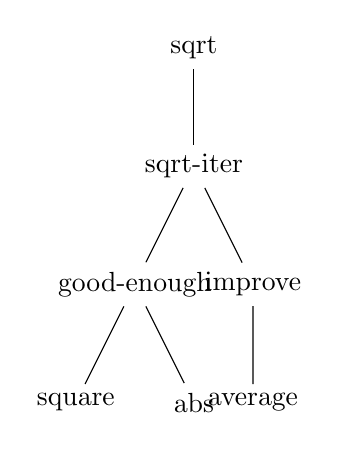
\begin{tikzpicture}[]
    \node {sqrt}
      child { node {sqrt-iter}
        child { node {good-enough}
          child { node {square} }
          child { node {abs} } }
        child { node {improve}
          child { node {average} } } } ;
\end{tikzpicture}
  \caption{Procedural decomposition of the \texttt{sqrt} program}
  \label{fig:1.2}
\end{figure}
          
            
The importance of this decomposition strategy is not simply that one
is dividing the program into parts.  After all, we could take any
large program and divide it into parts -- the first ten lines, the next
ten lines, the next ten lines, and so on.  Rather, it is crucial that
each procedure accomplishes an identifiable task that can be used as a
module in defining other procedures.  For example, when we define the
\texttt{good-enough?} procedure in terms of \texttt{square}, we are able to
regard the \texttt{square} procedure as a ``black box.''  We are not at
that moment concerned with \textit{how} the procedure computes its
result, only with the fact that it computes the square.  The details
of how the square is computed can be suppressed, to be considered at a
later time.  Indeed, as far as the \texttt{good-enough?} procedure is
concerned, \texttt{square} is not quite a procedure but rather an
abstraction of a procedure, a so-called \idef{procedural abstraction}.
At this level of abstraction, any procedure that computes the square
is equally good.

Thus, considering only the values they return, the following two
procedures for squaring a number should be indistinguishable.  Each
takes a numerical argument and produces the square of that number as
the value. \footnote{It is not even clear which of these procedures is
  a more efficient implementation.  This depends upon the hardware
  available.  There are machines for which the ``obvious''
  implementation is the less efficient one.  Consider a machine that
  has extensive tables of logarithms and antilogarithms stored in a
  very efficient manner.}

\begin{schemedisplay}
(define (square x) (* x x))

(define (square x) 
  (exp (double (log x))))

(define (double x) (+ x x))
\end{schemedisplay}

So a procedure definition should be able to suppress detail.  The
users of the procedure may not have written the procedure themselves,
but may have obtained it from another programmer as a black box.  A
user should not need to know how the procedure is implemented in order
to use it.

\subsubsection*{Local names}

One detail of a procedure's implementation that should not matter to
the user of the procedure is the implementer's choice of names for the
procedure's formal parameters.  Thus, the following procedures should
not be distinguishable:

\begin{schemedisplay}
(define (square x) (* x x))

(define (square y) (* y y))
\end{schemedisplay}

This principle -- that the meaning of a procedure should be independent
of the parameter names used by its author -- seems on the surface to be
self-evident, but its consequences are profound.  The simplest
consequence is that the parameter names of a procedure must be local
to the body of the procedure.  For example, we used \texttt{square} in
the definition of \texttt{good-enough?} in our square-root procedure:

\begin{schemedisplay}
(define (good-enough? guess x)
  (< (abs (- (square guess) x)) 0.001))
\end{schemedisplay}

The intention of the author of \texttt{good-enough?} is to determine if
the square of the first argument is within a given tolerance of the
second argument.  We see that the author of \texttt{good-enough?} used
the name \texttt{guess} to refer to the first argument and \texttt{x} to
refer to the second argument.  The argument of \texttt{square} is \texttt{guess}.  If the author of \texttt{square} used \texttt{x} (as above)
to refer to that argument, we see that the \texttt{x} in \texttt{good-enough?} must be a different \texttt{x} than the one in \texttt{square}.  Running the procedure \texttt{square} must not affect the value
of \texttt{x} that is used by \texttt{good-enough?}, because that value of
\texttt{x} may be needed by \texttt{good-enough?} after \texttt{square} is done
computing.

If the parameters were not local to the bodies of their respective
procedures, then the parameter \texttt{x} in \texttt{square} could be
confused with the parameter \texttt{x} in \texttt{good-enough?}, and the
behavior of \texttt{good-enough?} would depend upon which version of
\texttt{square} we used.  Thus, \texttt{square} would not be the black box
we desired.

A formal parameter of a procedure has a very special role in the
procedure definition, in that it doesn't matter what name the formal
parameter has.  Such a name is called a \idef{bound variable}, and we
say that the procedure definition \idef{binds} its formal parameters.
The meaning of a procedure definition is unchanged if a bound variable
is consistently renamed throughout the definition.\footnote{The
concept of consistent renaming is actually subtle and difficult to
define formally.  Famous logicians have made embarrassing errors
here.}  If a variable is not bound, we say that it is \idef{free}.  The
set of expressions for which a binding defines a name is called the
\idef{scope} of that name.
In a procedure definition, the bound variables
declared as the \idef{formal parameters} of the procedure have the body of
the procedure as their scope.

In the definition of \texttt{good-enough?} above, \texttt{guess} and \texttt{x} are
bound variables but \texttt{<}, \texttt{-}, \texttt{abs}, and \texttt{square} are free.
The meaning of \texttt{good-enough?} should be independent of the names we
choose for \texttt{guess} and \texttt{x} so long as they are distinct and
different from \texttt{<}, \texttt{-}, \texttt{abs}, and \texttt{square}.  (If we renamed
\texttt{guess} to \texttt{abs} we would have introduced a bug by \idef{capturing}
the variable \texttt{abs}.  It would have changed from free to bound.)  The
meaning of \texttt{good-enough?} is not independent of the names of its
free variables, however.  It surely depends upon the fact (external to
this definition) that the symbol \texttt{abs} names a procedure for
computing the absolute value of a number.  \texttt{Good-enough?} will
compute a different function if we substitute \texttt{cos} for \texttt{abs} in
its definition.

\subsubsection*{Internal definitions and block structure}


We have one kind of name isolation available to us so far: The formal
parameters of a procedure are local to the body of the procedure.  The
square-root program illustrates another way in which we would like to
control the use of names.  The existing program consists of separate
procedures:

\begin{schemedisplay}
(define (sqrt x)
  (sqrt-iter 1.0 x))
(define (sqrt-iter guess x)
  (if (good-enough? guess x)
      guess
      (sqrt-iter (improve guess x) x)))
(define (good-enough? guess x)
  (< (abs (- (square guess) x)) 0.001))
(define (improve guess x)
  (average guess (/ x guess)))
\end{schemedisplay}

The problem with this program is that the only procedure that is
important to users of \texttt{sqrt} is \texttt{sqrt}.  The other
procedures (\texttt{sqrt-iter}, \texttt{good-enough?}, and
\texttt{improve}) only clutter up their minds.  They may not define
any other procedure called \texttt{good-enough?} as part of another
program to work together with the square-root program, because
\texttt{sqrt} needs it.  The problem is especially severe in the
construction of large systems by many separate programmers.  For
example, in the construction of a large library of numerical
procedures, many numerical functions are computed as successive
approximations and thus might have procedures named
\texttt{good-enough?} and \texttt{improve} as auxiliary procedures.
We would like to localize the subprocedures, hiding them inside
\texttt{sqrt} so that \texttt{sqrt} could coexist with other
successive approximations, each having its own private
\texttt{good-enough?} procedure.  To make this possible, we allow a
procedure to have internal definitions that are local to that
procedure.  For example, in the square-root problem we can write

\begin{schemedisplay}
(define (sqrt x)
  (define (good-enough? guess x)
    (< (abs (- (square guess) x)) 0.001))
  (define (improve guess x)
    (average guess (/ x guess)))
  (define (sqrt-iter guess x)
    (if (good-enough? guess x)
        guess
        (sqrt-iter (improve guess x) x)))
  (sqrt-iter 1.0 x))
\end{schemedisplay}

Such nesting of definitions, called \idef{block structure},
is basically the right solution to the simplest 
name-packaging problem.  But there is a better idea lurking here.  In
addition to internalizing the definitions of the auxiliary procedures,
we can simplify them.  Since \texttt{x} is bound in the definition of
\texttt{sqrt}, the procedures \texttt{good-enough?}, \texttt{improve}, and
\texttt{sqrt-iter}, which are defined internally to \texttt{sqrt}, are in the
scope of \texttt{x}.  Thus, it is not necessary to pass \texttt{x} explicitly to
each of these procedures.  Instead, we allow \texttt{x} to be a free
variable in the internal definitions, as shown below. Then \texttt{x}
gets its value from the argument with which the enclosing
procedure \texttt{sqrt} is called.  This discipline is called \idef{lexical
scoping}.\footnote{Lexical
scoping dictates that free variables in a procedure are taken to refer to
bindings made by enclosing procedure definitions;
that is, they are looked up in
the environment in which the procedure was defined.  We will see how
this works in detail in chapter \ref{chap:3} when we study environments and the
detailed behavior of the interpreter.}

\begin{schemedisplay}
(define (sqrt x)
  (define (good-enough? guess)
    (< (abs (- (square guess) x)) 0.001))
  (define (improve guess)
    (average guess (/ x guess)))
  (define (sqrt-iter guess)
    (if (good-enough? guess)
        guess
        (sqrt-iter (improve guess))))
  (sqrt-iter 1.0))
\end{schemedisplay}

We will use block structure extensively to help us break up large
programs into tractable pieces. \footnote{Embedded definitions must
  come first in a procedure body.  The management is not responsible
  for the consequences of running programs that intertwine definition
  and use.}

The idea of block structure originated with the programming language
Algol 60.  It appears in most advanced programming languages and is an
important tool for helping to organize the construction of large
programs.

